\section{Introduction}

The first work now considered to be in the field of Artificial Intelligence (AI) was done by McCulloch and Pitts in 1943 \cite{McCulloch1943}.
They took inspiration from neurons in the brain and applied logic to their state of being either activated or not, including a switch determined by the activation of other neurons.
The term artificial intelligence itself was coined in 1956 by McCarthy by organizing a two-month workshop in Dartmouth \cite{McCarthy1955}.

After early great expectations on artificial intelligence without delivering promised results, the field got less attention.
A famous quote from Herbert Simon in 1957 states: 
\begin{quotation}
    It is not my aim to surprise or shock you – but the simplest way I can summarize is to say that there are now in the world machines that think, that learn and that create. Moreover, their ability to do these things is going to increase rapidly until – in a visible future – the range of problems they can handle will be coextensive with the range to which the human mind has been applied.
\end{quotation}

Over decades several advances have been made.
After another period of high investments in the 1980s without meeting the ambitious goals the so called "AI Winter" set in, which became apparent by lack of interest and funding.

In recent times however research and application of these techniques are again attracting more attention.
This is due to some factors prevalent in current times.
On one hand it is the shear amount of computing power which is now standard in computers.
Even home computers are nowadays capable of training models of remarkable complexity.

On the other hand the amount of data which is available due to the internet is easing the training for various tasks.
To train a model for a specific task suitable data is needed to make correct predictions on never seen data (generalization).
Since data is available in great amount\footnote{Several databases exist for research, training and evaluation.
A list of databases be inspected at \url{https://srp.klawr.de/\#1}}.

Therefore artificial intelligence is getting more attention in research and more and more practical fields are considering this technique as solution for various problems.
If recent enthusiasm are just excessive expectations, or if the "last invention of humankind" \cite{Good1965} is near remains to be seen.

The term artificial intelligence is used to describe machines performing tasks which are characteristic of human intelligence.
This being a relatively vague description the substantiation may be more fitting, going down to deep learning as a goal in this work.
This correlation is shown in figure \ref{fig:ai_ml_dl}.

\begin{figure}
    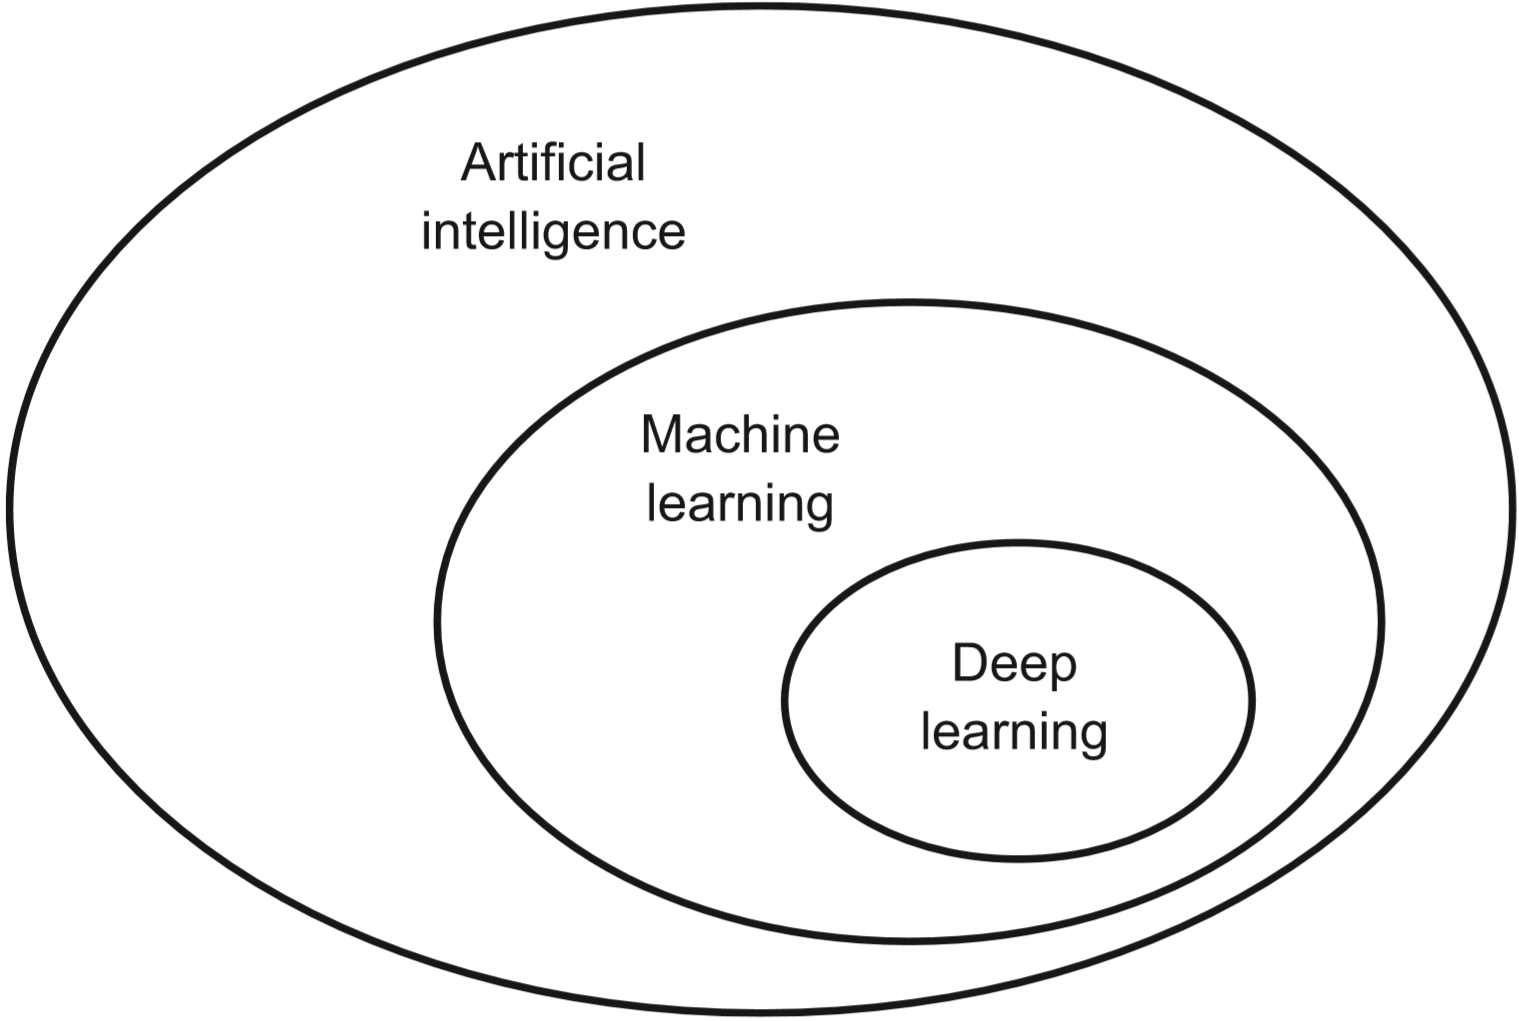
\includegraphics[width=0.5\textwidth]{images/ai_ml_dl.png}
    \caption{Artificial intelligence, machine learning and deep learning from \cite[p.4]{Chollet2017}}
    \label{fig:ai_ml_dl}
\end{figure}

In this project I want to introduce machine learning to the field of kinematics for two dimensional sketching and prototyping with \name{deepmech}.
The first solution implemented in this project takes images as input and outputs the respective type of handwritten mechanical symbols.
The models created by the presented approach are small and mostly language agnostic, which is provided by the usage of the popular Keras \cite{Chollet} library on top of TensorFlow \cite{Google}.

Simple demonstrations are done using JavaScript, connecting to an emerging field in kinematics using web technologies like \name{mec2}\footnote{\url{https://github.com/goessner/mec2}} \cite{Goessner2019} and \name{mecEdit}\footnote{\url{https://mecedit.com}} \cite{Uhlig2019}.
For training of the actual model the Python implementation of TensorFlow is used, because of better utilization of the GPU using CUDA \cite{nvidia2019} as backend which results in faster training.
Thanks to mostly language agnostic model descriptions this allows for seamless transitions between different approaches.

Before showing how deepmech was developed, the basics of machine learning shall be covered, showing some simple examples as introduction and by doing so introduce common terminology used in this paper.
In chapter 3 the concepts are extended by introducing neural networks, which are the key to implement the workings of machine learning into practical models.
Another topic which has to be covered is data generation. Data is a major part of training statistical models, so the data generation and augmentation is done in chapter 4.
Next the first working model will be discussed.
All major components will be examined in further detail to get a better understanding of every part.
The 6. chapter is about the tuning of said model to optimize the accuracy and minimize the size of the model which will be loaded in future applications.
Then the project is ended with a conclusion which will discuss the findings in further detail.
